\subsection{EXTENSIONS}

DEFINITION 1. Let F and G be two groups. An extension of G by F is a triple \(\mathcal{E} = (\mathrm{E}, i, p)\) , where E is a group, \(i\) an injective homomorphism of F into E and \(p\) a surjective homomorphism of E onto G such that \(\operatorname{Im}(i) = \operatorname{Ker}(p)\) . A homomorphism \(s: \mathrm{G} \to \mathrm{E}\) (resp. \(r: \mathrm{E} \to \mathrm{F}\) ) such that \(p \circ s = \operatorname{Id}_{\mathbf{G}}\) (resp. \(r \circ i = \operatorname{Id}_{\mathbf{F}}\) ) is called a section (resp. retraction) of the extension \(\mathcal{E}\) .

An extension \(\mathcal{E} = (\mathrm{E}, i, p)\) of \(\mathbf{G}\) by \(\mathbf{F}\) is often denoted by the diagram \(\mathcal{E}: \mathrm{F} \xrightarrow{i} \mathrm{E} \xrightarrow{p} \mathrm{G}\) , in which \(i\) and \(p\) are sometimes omitted if no confusion can arise. It is sometimes said simply that the group \(\mathbf{E}\) is an extension of \(\mathbf{G}\) by \(\mathbf{F}\) .

For a group E to be an extension of G by F, it is necessary and sufficient that it contain a normal subgroup \(F'\) isomorphic to F such that the quotient group \(E/F'\) is isomorphic to G.

An extension \(\mathcal{E}\colon\mathrm{F}\xrightarrow{i}\mathrm{E}\xrightarrow{p}\mathrm{G}\) is called central if the image \(i(\mathrm{F})\) is contained in the centre of E; this is only possible if F is commutative.

Let \(\mathcal{E}:\mathrm{F}\xrightarrow{i}\mathrm{E}\xrightarrow{p}\mathrm{G}\) and \(\mathcal{E}':\mathrm{F}\xrightarrow{i'}\mathrm{E}'\xrightarrow{p'}\mathrm{G}\) be two extensions of G by F. A morphism of \(\mathcal{E}\) into \(\mathcal{E}'\) is a homomorphism \(u:\mathrm{E}\to\mathrm{E}'\) such that \(p'\circ u=p\) and \(u\circ i=i'\) , or, in other words, such that the following diagram is commutative:

\pandocbounded{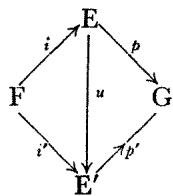
\includegraphics[keepaspectratio]{images/part001_e41623d9.jpg}}

PROPOSITION 1. Let \(\mathcal{E}: F \xrightarrow{i} E \xrightarrow{p} G\) and \(\mathcal{E}': F \xrightarrow{i'} E' \xrightarrow{p'} G\) be extensions of \(G\) by \(F\) . If \(u: E \to E'\) is a morphism of \(\mathcal{E}\) into \(\mathcal{E}'\) , \(u\) is an isomorphism of \(E\) onto \(E'\) and \(u^{-1}\) is a morphism of \(\mathcal{E}'\) into \(\mathcal{E}\) .

Let \(x \in E\) be such that \(u(x) = e\) . Then \(p(x) = p'(u(x)) = e\) , whence \(x \in i(F)\) . Let \(y \in F\) be such that \(x = i(y)\) ; then \(i'(y) = u(i(y)) = e\) . As \(i'\) is injective, \(y = e\) and \(x = e\) . Therefore \(u\) is injective. By virtue of §4, no. 6, Corollary 1 to Proposition 7, \(u\) is surjective since \(u(i(F)) = i'(F)\) . The last assertion is immediate.

In other words, the extensions \(\mathcal{E}\) and \(\mathcal{E}'\) are isomorphic if and only if there exists a morphism of \(\mathcal{E}\) into \(\mathcal{E}'\) .

Let \(\mathbf{F}\) and \(\mathbf{G}\) be two groups and write \(\mathbf{E}_0 = \mathbf{F} \times \mathbf{G}\) ; let \(i: \mathbf{F} \to \mathbf{E}_0\) be the canonical injection and \(p: \mathbf{E}_0 \to \mathbf{G}\) be the canonical projection. Every extension of \(\mathbf{G}\) by \(\mathbf{F}\) isomorphic to the extension \(\mathcal{E}_0: \mathbf{F} \xrightarrow{i} \mathbf{E}_0 \xrightarrow{p} \mathbf{G}\) is called a trivial extension.

PROPOSITION 2. Let \(\mathcal{E}:\mathrm{F}\xrightarrow{i}\mathrm{E}\xrightarrow{p}\mathrm{G}\) be an extension of \(\mathrm{G}\) by \(\mathrm{F}\) . The following conditions are equivalent:

\begin{enumerate}
\def\labelenumi{(\roman{enumi})}
\item
  \(\mathcal{E}\) is a trivial extension;
\item
  \(\mathcal{E}\) has a retraction \(r\) ;
\item
  \(\mathcal{E}\) has a section \(s\) such that \(s(\mathbf{G})\) is contained in the centralizer of \(i(\mathbf{F})\) .
\end{enumerate}

Clearly (i) implies (ii) and (iii). If (ii) holds, the mapping \((r, p): \mathbf{E} \to \mathbf{F} \times \mathbf{G}\) is a morphism of \(\mathcal{E}\) into \(\mathcal{E}_0\) , whence (i). If (iii) holds, the homomorphism of \(\mathbf{F} \times \mathbf{G}\) into \(\mathbf{E}\) corresponding to \((i, s)\) ( \(\S 4\) , no. 9, Proposition 12) is a morphism of \(\mathcal{E}_0\) into \(\mathcal{E}\) , whence (i).

It may be that an extension \(\mathcal{E}:\mathbf{F}\to\mathbf{E}\to\mathbf{G}\) is not trivial and yet the group \(\mathbf{E}\) is isomorphic to \(\mathbf{F}\times\mathbf{G}\) (Exercise 6).

DEFINITION 2. Let F and G be two groups and \(\tau\) a homomorphism of G into the automorphism group of F. Write \(\tau(g)(f) = {}^g f\) for \(g \in G\) and \(f \in F\) . The set \(\mathbf{F} \times \mathbf{G}\) with the law of composition

\[
((f, g), (f ^ {\prime}, g ^ {\prime})) \mapsto (f, g) \cdot_ {\tau} (f ^ {\prime}, g ^ {\prime}) = (f. ^ {g} f ^ {\prime}, g g ^ {\prime})\tag{1}
\]

is called the external semi-direct product of G by F relative to \(\tau\) .

The external semi-direct product of G by F relative to \(\tau\) is denoted by \(F \times_{\tau} G\) .

PROPOSITION 3. The external semi-direct product \(\mathbf{F} \times_{\tau} \mathbf{G}\) is a group. The mappings \(i: \mathbf{F} \to \mathbf{F} \times_{\tau} \mathbf{G}\) defined by \(i(f) = (f, e)\) , \(p: \mathbf{F} \times_{\tau} \mathbf{G} \to \mathbf{G}\) defined by \(p(f, g) = g\) , and \(s: \mathbf{G} \to \mathbf{F} \times_{\tau} \mathbf{G}\) defined by \(s(g) = (e, g)\) are group homomorphisms. The triple \((\mathbf{F} \times_{\tau} \mathbf{G}, i, p)\) is an extension of \(\mathbf{G}\) by \(\mathbf{F}\) and \(s\) is a section of the extension.

We have:

\[
\begin{array}{r l} ((f, g) \cdot_ {\tau} (f ^ {\prime}, g ^ {\prime})) \cdot_ {\tau} (f ^ {\prime \prime}, g ^ {\prime \prime}) & = (f. ^ {g} f ^ {\prime}, g g ^ {\prime}) \cdot_ {\tau} (f ^ {\prime \prime}, g ^ {\prime \prime}) \\ & = (f. ^ {g} f ^ {\prime}. ^ {g g ^ {\prime}} f ^ {\prime \prime}, g g ^ {\prime} g ^ {\prime \prime}); \\ (f, g) \cdot_ {\tau} ((f ^ {\prime}, g ^ {\prime}) \cdot_ {\tau} (f ^ {\prime \prime}, g ^ {\prime \prime})) & = (f, g) \cdot_ {\tau} (f ^ {\prime}. ^ {g ^ {\prime}} f ^ {\prime \prime}, g ^ {\prime} g ^ {\prime \prime}) \\ & = (f. ^ {g} (f ^ {\prime}. ^ {g ^ {\prime}} f ^ {\prime \prime}), g g ^ {\prime} g ^ {\prime \prime}). \end{array}
\]

Now \({}^{g}(f'.{}^{g'}f'') = {}^{g}f'.{}^{gg'}f''\) , which shows that the law of composition defined by (1) is associative. The element \((e, e)\) is the identity under this law. The element \((f, g)\) admits as inverse \((^{g^{-1}}f^{-1}, g^{-1})\) . Hence the law of composition on \(F \times_{\tau} G\) is a group law. The other assertions are immediate.

Using the notation of Proposition 3, \(E_{\tau}\) will denote the extension

\[
\mathrm{F} \xrightarrow {i} \mathrm{F} \times_ {\tau} \mathrm{G} \xrightarrow {p} \mathrm{G}.
\]

Let \(\mathcal{E}'\colon F\stackrel{i'}{\to}E'\stackrel{p'}{\to}G\) be an extension of \(G\) by \(F\) and \(s'\colon G\to E'\) a section of \(\mathcal{E}'\) . We define an operation \(\tau\) of \(G\) on the group \(F\) by:

\[
i ^ {\prime} (\tau (g, f)) = s ^ {\prime} (g) i ^ {\prime} (f) s ^ {\prime} (g) ^ {- 1} = \operatorname{Int} (s ^ {\prime} (g)) (i ^ {\prime} (f)).\tag{2}
\]

PROPOSITION 4. With the above notation, there exists one and only one isomorphism \(u\) of \(\mathcal{E}_{\tau}\) onto \(\mathcal{E}'\) such that \(u \circ s = s'\) .

\((f, g) = (f, e) \cdot_ {\tau} (e, g) = i(f).s(g)\) . Therefore, if u is a solution to the problem, of necessity \(u(f,g)=i'(f).s'(g)\) , whence the uniqueness of u. We prove the existence. We write \(u(f,g)=i'(f).s'(g)\) . Then

\[
\begin{array}{r l} u (f, g) \cdot u (f ^ {\prime}, g ^ {\prime}) & = i ^ {\prime} (f) s ^ {\prime} (g) i ^ {\prime} (f ^ {\prime}) s ^ {\prime} (g ^ {\prime}) \\ & = i ^ {\prime} (f) (s ^ {\prime} (g) i ^ {\prime} (f ^ {\prime}) s ^ {\prime} (g) ^ {- 1}) s ^ {\prime} (g) s ^ {\prime} (g ^ {\prime}) \\ & = i ^ {\prime} (f) i ^ {\prime} (\tau (g, f ^ {\prime})) \cdot s ^ {\prime} (g) s ^ {\prime} (g ^ {\prime}) \\ & = i ^ {\prime} (f \cdot \tau (g, f ^ {\prime})) \cdot s ^ {\prime} (g g ^ {\prime}) \\ & = u ((f, g) \cdot_ {\tau} (f ^ {\prime}, g ^ {\prime})). \end{array}
\]

Therefore, \(u\) is a homomorphism of \(\mathbf{F} \times_{\tau} \mathbf{G}\) into \(\mathbf{E}'\) . Obviously \(u \circ i = i'\) , \(p' \circ u = p\) and \(u \circ s = s'\) .

Remark. The definition of the operation \(\tau\) by formula (2) depends on the extension \(\mathcal{E}'\) and the section \(s'\) . When F is commutative, the operation \(\tau\) does not depend on \(s'\) . For \(\operatorname{Int}(s'(g)) \mid i'(F)\) depends then only on the coset of \(s'(g)\) mod. \(i'(F)\) .

More generally, let \(\mathcal{E}:\mathrm{F}\to \mathrm{E}\to \mathrm{G}\) be an extension of \(\mathbf{G}\) by a commutative group \(\mathbf{F}\) (it is not assumed that \(\mathcal{E}\) admits a section). The group \(\mathbf{E}\) operates on \(\mathbf{F}\) by inner automorphisms, this image is trivial on the image of \(\mathbf{F}\) and hence defines an operation of \(\mathbf{G}\) on \(\mathbf{F}\) . If \(\mathcal{E}\) admits a section, this operation is that defined by formula (2).

COROLLARY. Let G be a group and H and K two subgroups of G such that H is normal, \(\mathbf{H} \cap \mathbf{K} = \{e\}\) and \(\mathbf{H} \cdot \mathbf{K} = \mathbf{G}\) . Let \(\tau\) be the operation of \(\mathbf{K}\) on \(\mathbf{H}\) by inner automorphisms of \(\mathbf{G}\) . The mapping \((h, k) \mapsto hk\) is an isomorphism of \(\mathbf{H} \times_{\tau} \mathbf{K}\) onto \(\mathbf{G}\) .

Under the hypotheses of this corollary, G is said to be the semi-direct product of K by H.

Examples. (1) Let G be a group and E a homogeneous principal G-set; let \(\Gamma\) denote the automorphism group of G. Let A be the set of permutations f of E with the following property:

There exists \(\gamma \in \Gamma\) such that \(f\) is a \(\gamma\) -morphism of \(\mathbf{E}\) into \(\mathbf{E}\) (that is, \(f(gb) = \gamma(g)f(b)\) for \(b \in \mathbf{E}\) and \(g \in \mathbf{G}\) ).

The above formula \(f(gb) = \gamma(g)f(b)\) shows that if \(f \in A\) there exists a unique \(\gamma \in \Gamma\) such that \(f\) is a \(\gamma\) -morphism, we shall denote it by \(p(f)\) .

Let \(f, f'\) be in A, \(\gamma = p(f), \gamma' = p(f')\) . Then, for all \(b \in E\) and all \(g \in G\) ,

\[
(f ^ {\prime} \circ f) (g b) = f ^ {\prime} (\gamma (g) f (b)) = \gamma^ {\prime} (\gamma (g)) f ^ {\prime} (f (b))
\]

which proves that \(f' \circ f \in \mathbf{A}\) and that \(p(f' \circ f) = p(f')p(f)\) . On the other hand, \(f(\gamma^{-1}(g)f^{-1}(b)) = gb\) , whence \(f^{-1}(gb) = \gamma^{-1}(g)f^{-1}(b)\) and \(f^{-1} \in \mathbf{A}\) . Thus \(\mathbf{A}\) is a subgroup of \(\mathfrak{S}_{\mathbf{E}}\) and \(p\) is a homomorphism of \(\mathbf{A}\) into \(\Gamma\) . The kernel of \(p\) is the set \(\operatorname{Aut}_{\mathbf{G}}(\mathbf{E})\) of automorphisms of the \(\mathbf{G}\) -set \(\mathbf{E}\) .

We fix \(a \in \mathbf{E}\) . We have defined in § 5, no. 6 an isomorphism \(\psi_a\) of \(\mathbf{G}^0\) onto \(\operatorname{Aut}_{\mathbf{G}}(\mathbf{E})\) such that \(\psi_a(x)(ga) = gxa\) for all \(g, x\) in \(\mathbf{G}\) . On the other hand, for \(\gamma \in \Gamma\) , let \(s_a(\gamma)\) be the permutation of \(\mathbf{E}\) defined by \(s_a(\gamma)(ga) = \gamma(g)a\) for all \(g \in \mathbf{G}\) ; it is immediately verified that \(s_a\) is a homomorphism of \(\Gamma\) into \(\mathbf{A}\) such that \(p \circ s_a = \operatorname{Id}_{\Gamma}\) . Thus \(\mathbf{G}^0 \xrightarrow{\psi_a} \mathbf{A} \xrightarrow{p} \Gamma\) is an extension of \(\Gamma\) by \(\mathbf{G}^0\) and \(s_a\) is a section of this extension. This extension and this section define an operation of \(\Gamma\) on \(\mathbf{G}^0\) , \(s_a(\Gamma)\) acting on \(\psi_a(\mathbf{G}^0)\) by inner automorphisms; we write this operation exponentially. We show that this operation is the natural operation (§ 3, no. 1, Example 3): for \(x, g\) in \(\mathbf{G}\) and \(\gamma \in \Gamma\) ,

\[
\begin{array}{r l} (\psi_ {a} (^ {\gamma} x)) (g a) & = (s _ {a} (\gamma) \circ \psi_ {a} (x) \circ s _ {a} (\gamma) ^ {- 1}) (g a) \\ & = (s _ {a} (\gamma) \circ \psi_ {a} (x)) (\gamma^ {- 1} (g) a) = s _ {a} (\gamma) (\gamma^ {- 1} (g) x a) \\ & = g \gamma (x) a = \psi_ {a} (\gamma (x)) g a \end{array}
\]

whence \({}^{\gamma}x = \gamma(x)\) .

Proposition 4 then shows that A is isomorphic to the semidirect product of \(\Gamma = \operatorname{Aut}(\mathbf{G})\) by \(\mathbf{G}^0\) under the natural operation of \(\operatorname{Aut}(\mathbf{G})\) on \(\mathbf{G}^0\) . Note that the isomorphism which we have constructed depends in general on the choice of the element \(a \in \mathbf{E}\) .

\begin{enumerate}
\def\labelenumi{(\arabic{enumi})}
\setcounter{enumi}{1}
\tightlist
\item
  *Let A be a commutative ring. The upper triangular group T(n, A) is the semi-direct product of the diagonal subgroup D(n, A) by the upper strict triangular group T1(n, A).*
\end{enumerate}

